\section{AttackTrees}

\begin{figure}[h]
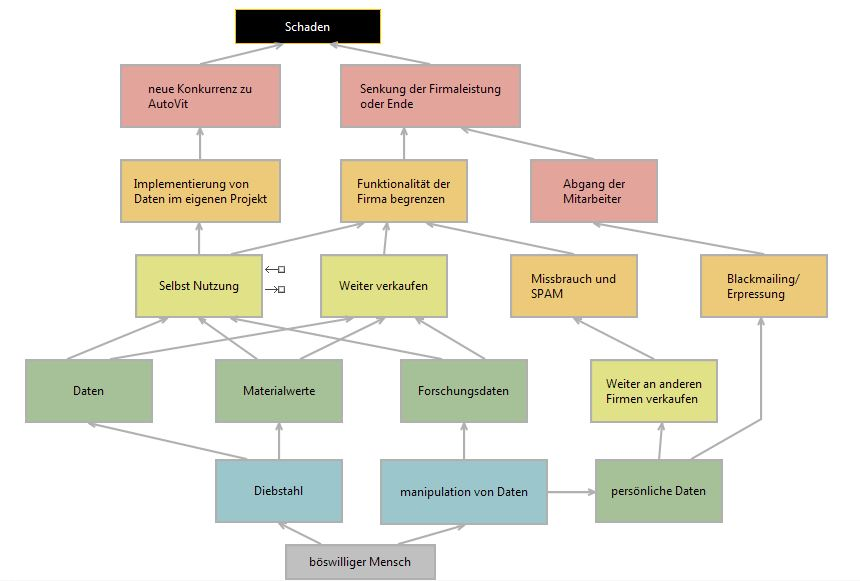
\includegraphics[scale=0.8, angle=90]{images/attacktree_boesermensch.jpg} 
\caption{Attack Tree - Böser Mensch}
\end{figure}

Das Diagramm veranschaulicht einen böswilligen Menschen, welcher mit den gegebenen Handlungen gewisse Folgen herbeiführen kann. Am Anfang steht eine Person, die zum einen durch Diebstahl oder durch die Manipulation von Daten auf diverse Objekte Einfluss nimmt, wie persönliche Daten oder Forschungsdaten. Dabei handelt es sich beispielsweise um Hardware, Möbel oder andere Vermögen der Firma. Daten, Materialwerte oder Forschungsdaten kann er selbst nutzen oder an Dritte weiterverkaufen. Die Implementierung von Daten im eigenen Projekt führt potentiell zur neuen Konkurrenz der eigenen Firma. Damit ist die Funktionalität der AutoVit Firma begrenzt und kann auch die Leistung senken.
\\
\\
Mit den persönlichen Daten ist die Person in der Lage, für eventuelle Erpressungen des Besitzers zu nutzen oder an Werbetreibende Firmen zu verkaufen. Wenn die Erpressung sehr stark ist, resultiert das in dem Abgang der Mitarbeiter. Die resultierenden Schäden können vom Abgang der Mitarbeiter, über neue Konkurrenz zur eigenen Firma, bis hin zur letztendlichen Schließung des Unternehmens führen.
